% GENERATED by scripts/make_figure1.py. DO NOT EDIT BY HAND.
% Regenerate in the pinned image; the generator needs scipy for the planning
% requirement, which is computed by scripts/audit_stats.py and never typed.
%
% Requires \usepackage{tikz} and \usetikzlibrary{arrows.meta} in the preamble.
%
% Provenance for every number here is paper/figures/fig1_values.json.
% NOT RENDERED OR VISUALLY INSPECTED: there is no LaTeX on the machine that
% generated this (probe job 11675341), so the first person to compile it must
% check it for clipping, overlap and label legibility.
\definecolor{fharm}{RGB}{140,45,20}
\definecolor{fben}{RGB}{125,178,219}
\definecolor{fneutral}{RGB}{110,110,110}
\definecolor{frule}{RGB}{60,60,60}

\begin{figure}[!t]
\centering
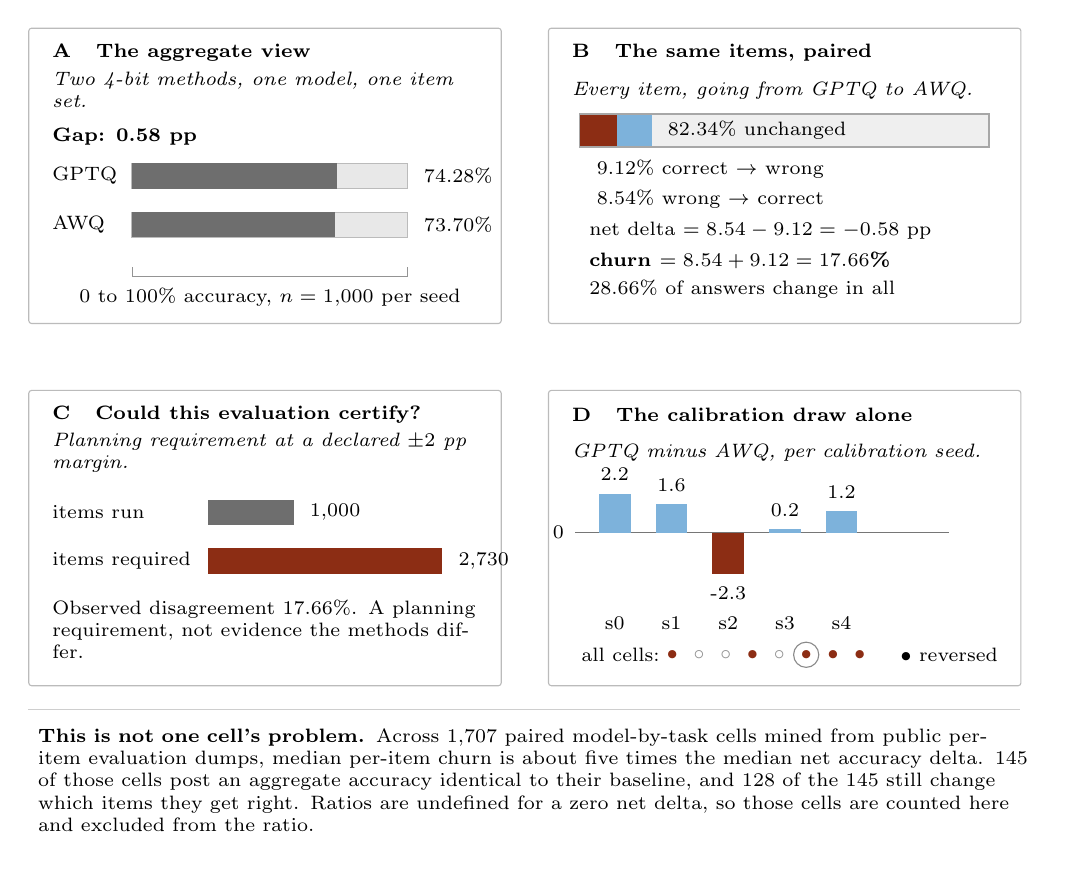
\begin{tikzpicture}[
  x=1cm, y=1cm, line width=0.5pt,
  font=\scriptsize,
  panel/.style={draw=frule!35, rounded corners=1pt, line width=0.4pt},
  ttl/.style={font=\scriptsize\bfseries, anchor=west},
  lbl/.style={font=\scriptsize, anchor=west},
  num/.style={font=\scriptsize, anchor=west},
]
\node[panel, minimum width=6.0cm, minimum height=3.75cm, anchor=south west] at (0.0,6.15) {};
\node[ttl] at (0.18,9.6) {A\quad The aggregate view};
\node[lbl, font=\scriptsize\itshape, text width=5.5cm] at (0.18,9.120000000000001) {Two 4-bit methods, one model, one item set.};
\node[lbl] at (0.18,8.03) {GPTQ};
\draw[fill=frule!12, draw=frule!35] (1.32,7.87) rectangle (4.82,8.19);
\draw[fill=fneutral, draw=none] (1.32,7.87) rectangle (3.9198000000000004,8.19);
\node[num, anchor=west] at (4.9,8.03) {74.28\%};
\node[lbl] at (0.18,7.41) {AWQ};
\draw[fill=frule!12, draw=frule!35] (1.32,7.25) rectangle (4.82,7.57);
\draw[fill=fneutral, draw=none] (1.32,7.25) rectangle (3.8995000000000006,7.57);
\node[num, anchor=west] at (4.9,7.41) {73.70\%};
\draw[frule!55, line width=0.4pt] (1.32,6.87) -- (1.32,6.75) -- (4.82,6.75) -- (4.82,6.87);
\node[font=\scriptsize, anchor=north] at (3.0700000000000003,6.73) {0 to 100\% accuracy, $n=1{,}000$ per seed};
\node[font=\scriptsize\bfseries, anchor=west] at (0.18,8.530000000000001) {Gap: 0.58 pp};
\node[panel, minimum width=6.0cm, minimum height=3.75cm, anchor=south west] at (6.6,6.15) {};
\node[ttl] at (6.779999999999999,9.6) {B\quad The same items, paired};
\node[lbl, font=\scriptsize\itshape, text width=5.5cm] at (6.779999999999999,9.120000000000001) {Every item, going from GPTQ to AWQ.};
\draw[fill=fharm, draw=none] (7.0,8.4) rectangle (7.47424,8.82);
\draw[fill=fben, draw=none] (7.47424,8.4) rectangle (7.91832,8.82);
\draw[fill=frule!8, draw=none] (7.91832,8.4) rectangle (12.2,8.82);
\draw[draw=frule!45] (7.0,8.4) rectangle (12.2,8.82);
\node[font=\scriptsize, anchor=west] at (7.99832,8.610000000000001) {82.34\% unchanged};
\node[lbl, anchor=west] at (7.0,8.120000000000001) {\textcolor{fharm}{$\blacksquare$} 9.12\% correct $\to$ wrong};
\node[lbl, anchor=west] at (7.0,7.74) {\textcolor{fben}{$\blacksquare$} 8.54\% wrong $\to$ correct};
\node[lbl, anchor=west] at (7.0,7.34) {net delta $= 8.54 - 9.12 = -0.58$ pp};
\node[lbl, anchor=west, font=\scriptsize\bfseries] at (7.0,6.960000000000001) {churn $= 8.54 + 9.12 = 17.66$\%};
\node[lbl, anchor=west] at (7.0,6.6000000000000005) {28.66\% of answers change in all};
\node[panel, minimum width=6.0cm, minimum height=3.75cm, anchor=south west] at (0.0,1.55) {};
\node[ttl] at (0.18,5.0) {C\quad Could this evaluation certify?};
\node[lbl, font=\scriptsize\itshape, text width=5.5cm] at (0.18,4.52) {Planning requirement at a declared $\pm2$ pp margin.};
\node[lbl] at (0.18,3.76) {items run};
\draw[fill=fneutral, draw=none] (2.28,3.5999999999999996) rectangle (3.3715750915750915,3.9199999999999995);
\node[num] at (3.4515750915750916,3.76) {1{,}000};
\node[lbl] at (0.18,3.1399999999999997) {items required};
\draw[fill=fharm, draw=none] (2.28,2.9799999999999995) rectangle (5.26,3.2999999999999994);
\node[num] at (5.34,3.1399999999999997) {2{,}730};
\node[lbl, text width=5.55cm, anchor=north west] at (0.18,2.77) {Observed disagreement 17.66\%. A planning requirement, not evidence the methods differ.};
\node[panel, minimum width=6.0cm, minimum height=3.75cm, anchor=south west] at (6.6,1.55) {};
\node[ttl] at (6.779999999999999,5.0) {D\quad The calibration draw alone};
\node[lbl, font=\scriptsize\itshape, text width=5.5cm] at (6.779999999999999,4.52) {GPTQ minus AWQ, per calibration seed.};
\draw[frule!70, line width=0.5pt] (6.949999999999999,3.5) -- (11.7,3.5);
\node[font=\scriptsize, anchor=east] at (6.93,3.5) {0};
\draw[fill=fben, draw=none] (7.249999999999999,3.5) rectangle (7.6499999999999995,3.997391304347826);
\node[font=\scriptsize, anchor=south] at (7.449999999999999,4.037391304347826) {2.2};
\node[font=\scriptsize, anchor=north] at (7.449999999999999,2.55) {s0};
\draw[fill=fben, draw=none] (7.97,3.5) rectangle (8.37,3.8617391304347826);
\node[font=\scriptsize, anchor=south] at (8.17,3.9017391304347826) {1.6};
\node[font=\scriptsize, anchor=north] at (8.17,2.55) {s1};
\draw[fill=fharm, draw=none] (8.69,3.5) rectangle (9.089999999999998,2.98);
\node[font=\scriptsize, anchor=north] at (8.889999999999999,2.94) {-2.3};
\node[font=\scriptsize, anchor=north] at (8.889999999999999,2.55) {s2};
\draw[fill=fben, draw=none] (9.41,3.5) rectangle (9.809999999999999,3.5452173913043477);
\node[font=\scriptsize, anchor=south] at (9.61,3.5852173913043477) {0.2};
\node[font=\scriptsize, anchor=north] at (9.61,2.55) {s3};
\draw[fill=fben, draw=none] (10.129999999999999,3.5) rectangle (10.529999999999998,3.771304347826087);
\node[font=\scriptsize, anchor=south] at (10.329999999999998,3.811304347826087) {1.2};
\node[font=\scriptsize, anchor=north] at (10.329999999999998,2.55) {s4};
\node[font=\scriptsize, anchor=west] at (6.8999999999999995,1.9500000000000002) {all cells:};
\node[font=\scriptsize, text=fharm] at (8.18,1.9500000000000002) {$\bullet$};
\node[font=\scriptsize, text=frule!55] at (8.52,1.9500000000000002) {$\circ$};
\node[font=\scriptsize, text=frule!55] at (8.86,1.9500000000000002) {$\circ$};
\node[font=\scriptsize, text=fharm] at (9.2,1.9500000000000002) {$\bullet$};
\node[font=\scriptsize, text=frule!55] at (9.54,1.9500000000000002) {$\circ$};
\node[font=\scriptsize, text=fharm] at (9.879999999999999,1.9500000000000002) {$\bullet$};
\draw[frule!60, line width=0.4pt] (9.879999999999999,1.9500000000000002) circle (0.16);
\node[font=\scriptsize, text=fharm] at (10.219999999999999,1.9500000000000002) {$\bullet$};
\node[font=\scriptsize, text=fharm] at (10.56,1.9500000000000002) {$\bullet$};
\node[font=\scriptsize, anchor=west] at (10.76,1.9500000000000002) {\ \ $\bullet$ reversed};
\draw[frule!25, line width=0.4pt] (0.0,1.25) -- (12.6,1.25);
\node[anchor=north west, text width=12.6cm, font=\scriptsize] at (0.0,1.1300000000000001) {\textbf{This is not one cell's problem.} Across 1{,}707 paired model-by-task cells mined from public per-item evaluation dumps, median per-item churn is about five times the median net accuracy delta. 145 of those cells post an aggregate accuracy identical to their baseline, and 128 of the 145 still change which items they get right. Ratios are undefined for a zero net delta, so those cells are counted here and excluded from the ratio.};
\end{tikzpicture}
\caption{\textbf{Near-equal aggregate accuracy does not certify interchangeable behavior.} One registered cell: Qwen2.5-7B on GSM8K, 4-bit GPTQ against 4-bit AWQ, paired on byte-identical calibration samples across five seeds. (A)~and~(B)~The aggregate gap of 0.58~pp is the small difference between two large opposing quantities summing to 17.66\%. (C)~The item count needed to certify equivalence at a declared $\pm2$~pp margin is a planning requirement computed at an assumed true difference of zero: it says the evaluation cannot support the claim, not that the methods differ. (D)~The sign changes with the calibration draw alone, and across the eight registered cells the winner reverses in 5 of 8. \textbf{Scope.} This cell is an illustrative example chosen because it is legible, and it is the most extreme of the eight: its churn-to-net-delta ratio is $30.4\times$ against a median of $12.7\times$ across the eight. All eight are shown in~(D) for that reason. The atlas figures in the panel above are observational and describe the public evaluation record rather than a census of compression.}
\label{fig:cancellation}
\end{figure}
